\chapter{Data Science Project - Dataset Analysis}

\section{The Data Supplied}
\paragraph{ }The data supplied was taken directly from \textit{Times of Malta} classified listing page on some of the days when the listings would go live from the 23\textsuperscript{rd} of April 2015 to the 24\textsuperscript{th} of October 2018. For mostly every week in that time frame, the data was either collected on a Monday or on a Wednesday or on both those days of the week. Each file contains the property listings for a whole week, thus there are duplicate entries in the dataset. Note that due to the differences in the time frame between each data point, if this data is going to be used for time series analysis then a sample needs to be taken with even time intervals to ensure accuracy of the tests.

\paragraph{ }The data collected is simply the \textit{html} code used to display the web page. This is available to anyone that has access to the website, thus anyone can have access to this data given the page was accessed on the specified date. Since anyone can book a classified advert on \textit{Times of Malta}, there is no guarantee that the information is correct or accurate, thus we cannot be certain that the prices of the properties listed on the classified page reflect the true market value of property in Malta set by experts in the field. However, this could still give us a good indication of the trend. 

\paragraph{ }With regards to data quality, the data provided is not complete as not all listings have information on the area of the house, whether or not the house has a garage or information on the type of property. However, from glancing at the raw data, it would seem that all entries have data on the location and price of the property. Since the data is extracted from the same system it must be consistent. Finally, when doing a study on the current property situation in Malta, data from 2015, 2016 or even 2017 will not be relevant or timely as the property marked has changed drastically in these past years in Malta. 

\section{Features of Interest}
\paragraph{ }The features of interest from the raw data were extracted with the task in mind of building a predictive model that would predict the expected price of the property given several features. Thus a sample was chosen from the provided dataset, in particular data from the beginning of August, September and October was chosen since these would reflect most accurately the current prices in the property market. 
\begin{itemize}
	\item \underline{Property ID}: This will be extracted from the \textit{name} variable in the \textit{html} code in order to have a unique ID referencing each entry.
	\item \underline{Location}: This categorical variable will store the location of the property. Since the price of property depends on the location, this would make a good predictor for the model.
	\item \underline{Property Type}: Another categorical variable which lists the type of property for sale. The categories are the following: house, penthouse, maisonette, apartment, farmhouse, villa, house of character, block or unknown.
	\item \underline{Plot Area}: This continuous quantitative variable stores the area of the land in square meters (thus its measured in a ratio scale). The plot area of the land should have a direct effect on the final price of the property, thus it should make a good predictor.
	\item \underline{Has Pool}: This dichotomous variable takes a value of 1 if the property listed has a pool and 0 otherwise.
	\item \underline{Has Garage}: This categorical variable has 3 categories; yes (1), no (0) and optional (2).
\end{itemize}

\section{Feature Extraction}
\paragraph{ }The data was extracted from the provided \textit{html} files by using the \textit{Python} package \textit{Beautiful Soup}. Once the property listings were found, the features were extracted using regular expressions and python's string manipulation libraries. The data in the location category was then arranged to ensure there's only 1 category per location. Finally, the duplicated entries were dropped, leaving a total of 1422 unique entries.

\section{Some Interesting Results}
\paragraph{ }Following some analysis on the extracted data, some interesting statements were initially made. Note that at this stage no statistical tests were done as this would be done later on in the analysis.

\paragraph{ }The first interesting conclusion was made on data to do with properties having pools. Firstly, the average value of properties with pools seems to be significantly larger than those without pools (as expected). In fact the average value of a property with a pool (regardless of location or size) was found to be \euro 818,616.07 while the average value of a property without a pool was found to be \euro 342,582. Furthermore, as can be seen in Figure \ref{fig::locPools}, at the time of the study, the locality selling the most properties with pools was Zejtun. 

\begin{figure}[!b]
	\begin{minipage}[b]{0.45\linewidth}
		\centering
		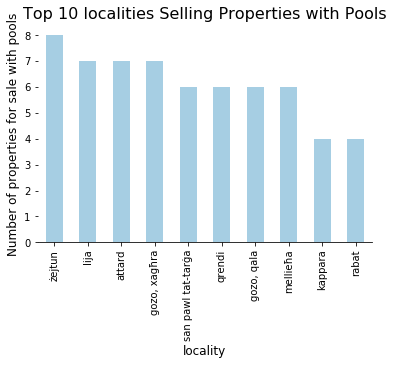
\includegraphics[width=\textwidth]{top_localities_pools}
		\caption[Pools]{Localities Selling the most Properties with Pools}
		\label{fig::locPools}
	\end{minipage}	
	\hspace{0.5cm}
	\begin{minipage}[b]{0.45\linewidth}
		\centering
		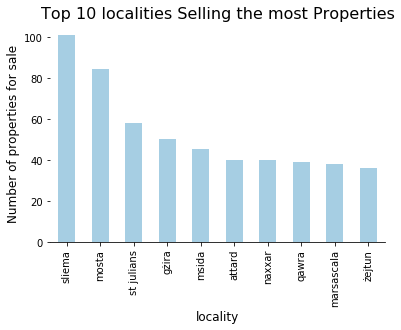
\includegraphics[width=\textwidth]{top_localities}
		\caption[Top Localities]{Localities Selling the most Properties}
		\label{fig::toplocalities}
	\end{minipage}	
\end{figure}

\paragraph{ }Another interesting result found during the data exploration stage was that currently on the market, Sliema is the locality that has the larges number of properties for sale. The top 10 localities selling properties can be seen in Figure \ref{fig::toplocalities}.

\paragraph{ }One of the questions that would be interesting to look at was \textit{``which locality has the most expensive land?"}. In order to answer this, the price per square meter of land for each property on the market was worked out by dividing the price by the area. The average was then worked out for each locality using the \textit{groupby} function and it was concluded that the most expensive land on the market right now is in Pender Gardens with an average of \euro 21,818.18 per square meter! Note that at this stage, properties with less than 35 square meters of land were removed as they were considered to be outliers.

\paragraph{ }The last interesting conclusion was made when analysing the property types. In general, as expected, the most expensive property type for sale was found to be the block of apartments which have an average price of \euro1,414,214. However it was interesting to note from looking at the density plots for the prices of apartments and houses (Figure \ref{fig::densities}) that prices for houses have greater variability than those of apartments. 

\begin{figure}[!t]
	\begin{minipage}[b]{0.45\linewidth}
		\centering
		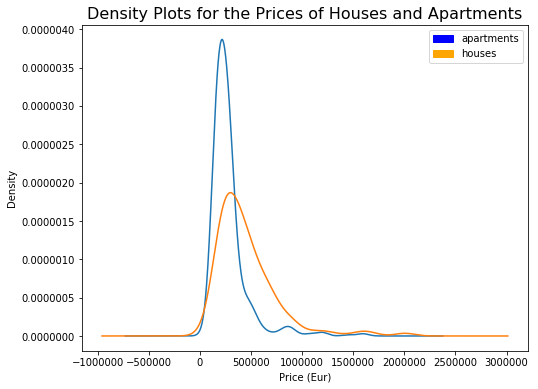
\includegraphics[width=\textwidth]{densities}
		\caption[Price Densities]{Density plots for the Prices of Houses and Apartments}
		\label{fig::densities}
	\end{minipage}	
	\hspace{0.5cm}
	\begin{minipage}[b]{0.45\linewidth}
		\centering
		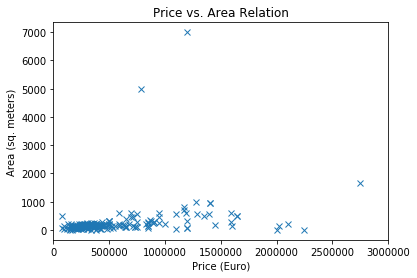
\includegraphics[width=\textwidth]{correlation}
		\caption[Correlation Plot]{Scatter Plot of Price vs. Area}
		\label{fig::correlation}
	\end{minipage}	
\end{figure}


\section{Identifying a Correlation}
\paragraph{ }The two variables that would seem to have an obvious correlation would be \textit{price} and \textit{area}. As the area of the land increases we would expect the price to increase too. In fact, having a quick look at the scatter plot in Figure \ref{fig::correlation} (after limiting the x-axis to remove some outliers) seems to confirm this. The outliers are points that are affected by the locality, it's obviously important not to remove these when building the model as the locality will be a key feature in the model.

\paragraph{ }A Pearson correlation test was then run and the data was found to have a correlation coefficient of 0.4861. The p-value of the test was found to be 1.84252e-15 which is less than 0.01, thus we are 99\% confident that the value is significant.

\section{Statistical Analysis}
\paragraph{ }Initially, tests for normality were done on the continuous variables, these tests are important as they would decide weather to use parametric tests or non-parametric tests in the future, as well as decide what kind of model to build to predict the prices of properties. In order to ensure the accuracy of the normality tests, two different tests were run; the Shapiro-Wilk normality test and the D'Agostino-Pearson omnibus test. Both these tests test the null hypothesis that the data is sampled from a normal distribution. Both these tests on both the continuous variables gave us the result that our data does not in fact come from an underlying normal distribution.

\paragraph{ }After running the normality tests, a test to see if there's a significant difference in the area of the property if it has a garage was run. It was decided to use the Mann Whitney-U Test with continuity correction as this is a non-parametric alternative to the independent sample t-test which tests for a significant difference in the medians of two independent groups. The test results showed with 99\% confidence that as expected, the average area of properties with a garage was significantly larger to those without a garage. Note that more details on the test can be seen in the markdown cells in the JuPyter notebook file `03 - Statistical Analysis'.

\section{The ANCOVA Regression Model}
\paragraph{ }The ANCOVA (Analyss of Covariance) regression model is similar to the ANOVA and OLS regression models, however it caters for categorical variables as predictors as well as covariates. The equation of this model is similar to that of the ANOVA model and can be seen in equation \ref{eq::ancova}.
\begin{equation}
\centering
\boldmath{y}=\mathbb{X}\boldmath{\beta}+\boldmath{\epsilon}
\label{eq::ancova}
\end{equation}
Where \boldmath{$y$} is an \textit{n}-vector of independent normally distributed responses, \boldmath{$\beta$} is a \textit{p}-vector of unknown regression parameters, \boldmath{$\epsilon$} is an \textit{n}-vector of error terms whose elements are assumed to follow a standard normal distribution and $\mathbb{X}$ is an (\textit{n}x\textit{p}) matrix whose values are both real values and dummy 0-1 indicators.

\paragraph{ }Similar to ANOVA regression, the equation for estimating the vector of parameters can be seen in equation \ref{eq::b}.
\begin{equation}
\centering
\boldmath{\hat{\beta}}=(\mathbb{X'X})^{-1}\mathbb{X}'\boldmath{y}
\label{eq::b}
\end{equation}
$\mathbb{X'X}$ has no inverse for the columns of each of the dummy variables since these are linearly dependent, thus a column from each of the dummy categorical variables must be dropped before performing the analysis, this is known as intrinsic aliasing.

\paragraph{ }The following assumptions were made when using the ANCOVA regression model:
\begin{itemize}
	\item The response variable must have a normal distribution.
	\item The response variable must be highly correlated with all quantitative predictors.
	\item There shouldn't be any multicollinearity between the quantitative predictors.
\end{itemize} 
Note that in this case, the response variable is not normally distributed, however it was decided to use this model anyway, keeping in mind that some degree of accuracy is lost due to this. A work-around solutions to this would be to use a different GLM (General Linear Model) that transforms the response variable using a link function. It was decided not to do this however, as this would greatly increase the complexity of the model which seems beyond the scope of this task.

\paragraph{ }The Model was first run to include \textit{location} as a predictor, however the majority of the coefficients turned out to not be significant, thus \textit{location} was removed and the model was built using \textit{area}, \textit{garage}, \textit{property type} and \textit{pool} as predictors. The final output shows us (from the adjusted $R^2$) value, that this model explains 62.5\% of the total variation of the dependent variable, which is what is to be expected when building models of this type.

\paragraph{ }The testing set was then used to test the accuracy of the implemented model and it was found that the model was quite inaccurate overall, having an average error of \euro299,444.35, rendering the model rather useless. Some solutions to building a better model of this type are to have a larger training set and to include interaction effects to the model with the hopes of building a more robust parsimonious model.